% Chapter 5

\chapter{Experimental setup} % Main chapter title

\label{expe} % For referencing the chapter elsewhere, use \ref{Chapter5}

% \lhead{Chapter 5. \emph{Experimental setup}} % This is for the header on each page - perhaps a shortened title

The proposed solution was tested in a study that required the definition of several conditions. First, it required to define the type of data to be collected. Then, the structure of data and the mechanisms of the collection were established. It was also important to identify the type of participants and divide them into groups to test different versions of the application. The versions of the application were distributed over a platform to let participants install them with ease. Finally, the study was set over a period of time, and the application was delivered to a broader audience.

%----------------------------------------------------------------------------------------
\section{Type of Data}
The required data to analyse and evaluate the solution came from the application. The data were automatically generated every time users interacted with the application. This type of data had a quantitative nature; therefore, it was possible to measure and analyse it from a statistical point of view. This type of data were collected from the start to the end of the period of the study.

Originally, AnkiDroid collects a lot of useful information, which is available to users in the form of statistics. These data are quantitative and give users a perspective on their progress based on the number of flashcards review, the number of sessions, the amount of time in sessions, and more. The application even forecasts the number of flashcards to be reviewed in the near future. This information was not collected for analysis since it provides a general overview of the usage from the perspective of users and lacks details related to the integrated game and the gamification elements.

\section{Collection and Structure of Data}
Quantitative data were generated in points where users interacted with the application, e.g. playing the game, selecting a deck, or reviewing flashcards. Each time an important interaction was done, the application processed the relevant information and sent it to an external server to save it. Therefore, it was necessary to define a scheme to format the information before storing it. The format was also aimed at facilitating the analysis and interpretation of results. Thus, quantitative information was grouped into four categories as seen in Table \ref{tab:info-type}.

\begin{table*}[!htb]
    \centering
    {\renewcommand{\arraystretch}{1}
        \begin{tabular}{|R{3cm}|R{6cm}|}
        \hline
        \multicolumn{1}{|>{\centering\arraybackslash}m{2cm}|}{\textbf{Category}} &
        \multicolumn{1}{>{\centering\arraybackslash}m{6cm}|}{\textbf{Description}} \\
        \hline
        Common & Details of time and user.\\
        \hline
        Game & Details about the game.\\
        \hline
        Gamification & Details of game elements. \\
        \hline
        Anki & Details of flashcards and decks. \\
        \hline
        \end{tabular}
    }
    \caption{Categories of quantitative information collected from the application.}
    \label{tab:info-type}
\end{table*}

The common category was meant to identify the time, date, and user that generated the interaction. This type of data was part of every relevant interaction in the application. The next category of information was related to the game; it included details about the score, cheat tricks, and state of the grid. The gamification category had to do with the added game elements to AnkiDroid. It included details about the number of coins, number of points, and names of the ankimals. Finally, the Anki category referred to details about the decks, flashcards, and revision times.

The categories of information were stored in the form of logs. Logs were a scheme to assemble and structure information from different categories based on the relevant interactions generated in the application. Logs were grouped into two main classes: game logs and Anki logs. Games logs contained information from the game category; however, some data from the gamification category was also registered in these logs. Anki logs contained information from Anki category with some data from the gamification category. Information about common category was recorded in both groups of logs as seen in Figure \ref{fig:categories-logs}.

\begin{figure}[htb]
    \vskip 5mm
        \begin{center}
            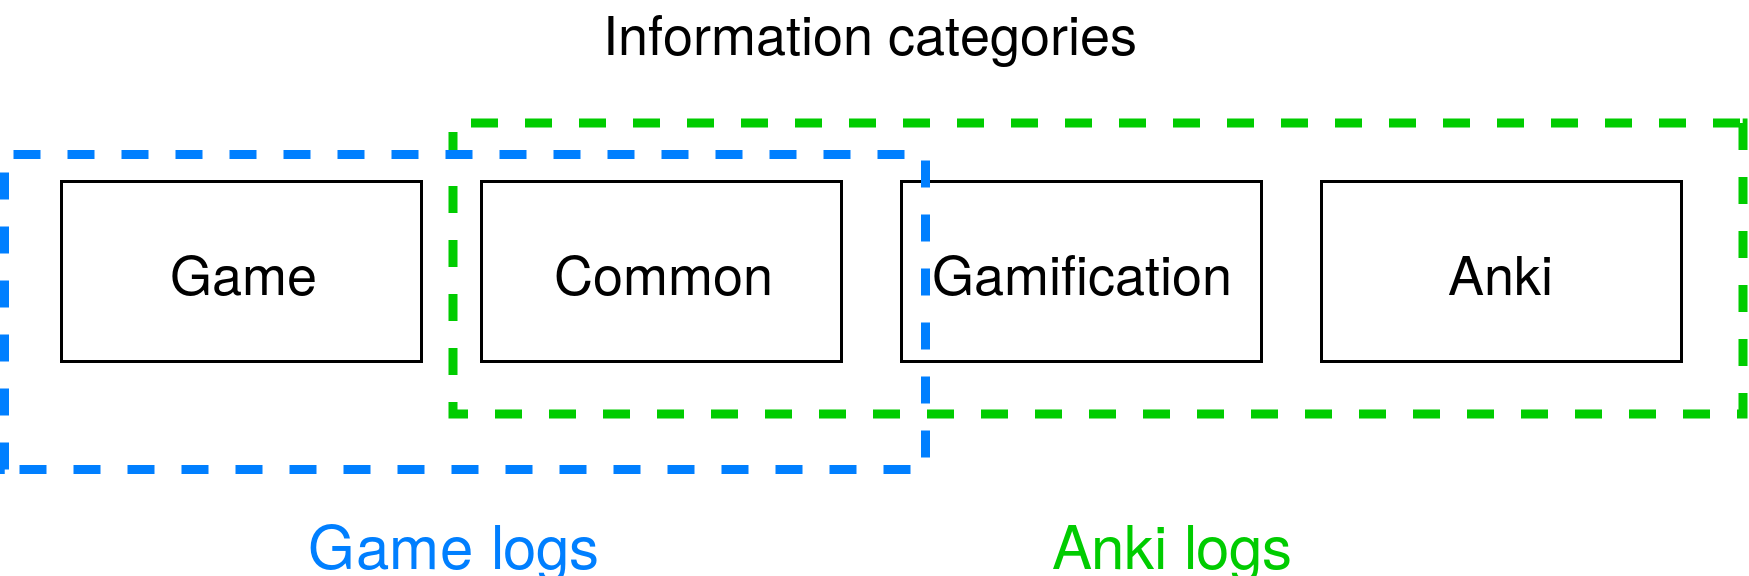
\includegraphics[scale=0.2]{./Figures/categories_logs.png}
            \caption{Types of logs and their relationships to information categories.}
            \label{fig:categories-logs}
        \end{center}
    \vskip -5mm
\end{figure}

Specifically speaking, there were 6 types of game logs and 9 types of Anki logs as shown in Table \ref{tab:log-types}. Game logs were generated in the game context. Something similar occurred with Anki logs; however, the design of the solution allowed one Anki log to be generated in the game context: Check leaderboard. This was possible because users could open the leadearboard either in the game context or in the Anki context. The reason for this design is that the leaderboard provided information about the social aspect. Despite the fact that the leaderboard displayed gamification data (points), users were not asked to do a specific action in Anki or the game contexts to see their positions.

\begin{table*}[!htb]
    \centering
    {\renewcommand{\arraystretch}{1}
        \begin{tabular}{ |c|c|c| }
            \hline
            \textbf{Type of log} & \textbf{Name of log} \\
            \hline
            \multirow{6}{3cm}{Game log} &  Game won\\
            & Game lost \\
            & Game restarted \\
            & Trick used \\
            & Trick failed \\
            & Switched to anki \\
            \hline
            \multirow{9}{3cm}{Anki log} &  Leaderboard checked\\
            & Custom study set \\
            & Flashcard answer revealed\\
            & Flashcard assessed \\
            & Deck selected \\
            & Ankimal rescued\\
            & Ankimal selected\\
            & Ankimal coloured\\
            & Switched to game \\
            \hline
        \end{tabular}
    }
    \caption{Types of logs collected from the application.}
    \label{tab:log-types}
\end{table*}

%----------------------------------------------------------------------------------------
\section{Participants}
\label{participants}
The study required recruiting a group of participants to use the application. The main requirement was to have an Android device to install the application. It was not necessary that participants had a specific profile. However, to maintain some level of homogeneity, the recruitment was done based on previous experience with AnkiDroid or other interfaces of Anki. The selected participants did not have any previous contact with Anki. Therefore, they were new to this educational tool and the modifications explained in chapter \ref{desi}.

Participants were recruited while the application was in the development phase. During this process, they were informed about the objective and duration of the study. Since they did not have any previous experience with AnkiDroid, they were taught about the objective, benefits, and functionalities of the application. In addition, they were also informed about the gamification features and the casual game. Participants were not forced to be part of the study from start to end. They were free to leave the study at any point as this situation provided additional insights into the application.

%----------------------------------------------------------------------------------------
\section{Groups of Participants}
As described in section \ref{game-integration}, the key difference between the proposed solution and others was the inclusion of a casual game. For this reason, the application was split into two versions. The first version had the causal game and all the other gamification elements; this version was named AnkiGame \citep{velasquez2018ankigame}. The second version did not have the integrated game, but the other gamification elements were available; this version was named AnkiPlay \citep{velasquez2018ankiplay}. Therefore, it was possible to analyse the effectiveness of the integration of a casual game as a means to increase user engagement.

Since there were two versions of the application, the participants were divided into two sets, each with six randomly selected members. The resulting sets were defined as the control group and the experimental group. Participants in the control group were given the AnkiPlay version, whereas participants in the second group were given the AnkiGame version as seen in Figure \ref{fig:participants-version}. None of the participants were told about the existence of the other version of the application. This decision was made to reduce any potential bias in the use of the application.

\begin{figure}[htb]
    \vskip 5mm
        \begin{center}
            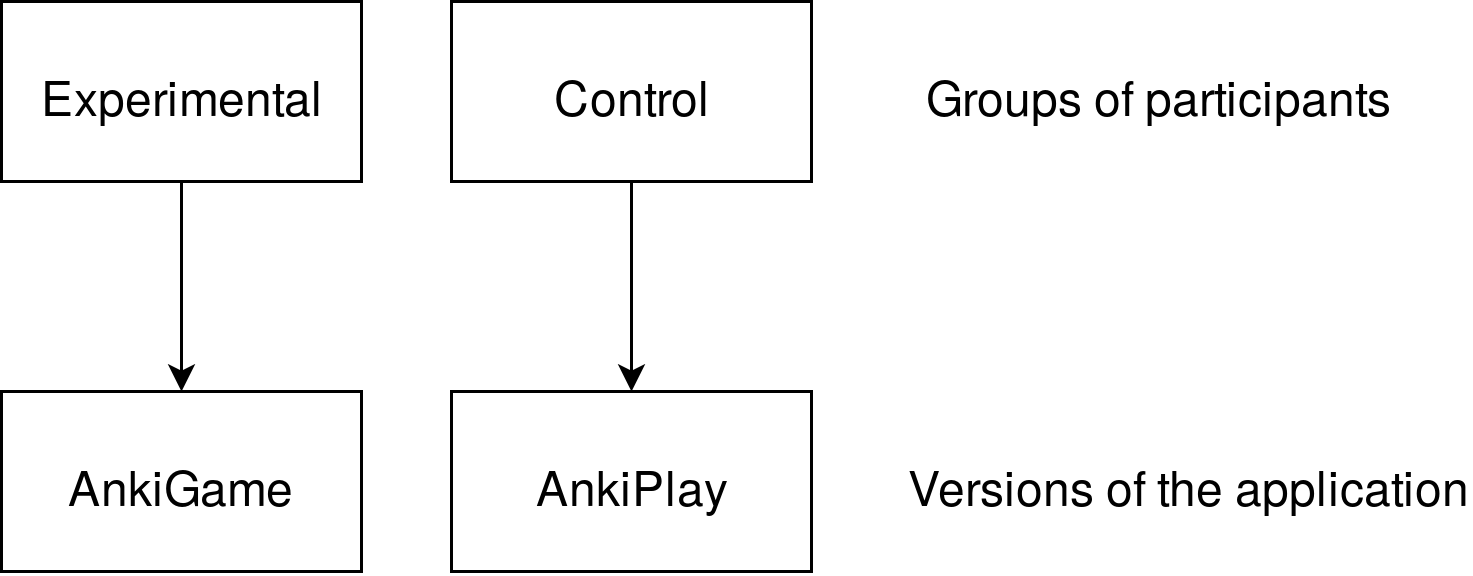
\includegraphics[scale=0.25]{./Figures/participants_version.png}
            \caption{Groups of participants and the assigned versions of the application.}
            \label{fig:participants-version}
        \end{center}
    \vskip -5mm
\end{figure}

%----------------------------------------------------------------------------------------
\section{Distribution of the Application}
The application was distributed in the Google Play Store. This platform allows having multiple versions of the same application in independent contexts. Therefore, it was possible to publish AnkiGame and AnkiPlay simultaneously. Thus, participants had an easy way to find and install the corresponding version on their devices. Another advantage of this platform is the different testing stages it offers. This feature was used to set a beta testing phase where potential issues were found and additional improvements were added to the application before making it available to participants.

In addition, Google Play Store allows making updates to correct bugs, add new features, or release new versions of an application. The updates are automatically installed in devices that already have the corresponding applications. Moreover, the distribution platform provides insights into the use and performance in the form of statistics. Users have the option to provide additional quantitative data by rating the application.

%----------------------------------------------------------------------------------------
\section{Duration of Study and Broader Audience}
The study was set to last four weeks when participants used the application and generated data. The study period was divided into two stages as seen in Figure \ref{fig:study-period}. The first stage lasted three weeks, and users were suggested to use the application at least during this period, but as explained in Section \ref{participants}, they were not forced to do so. At the end of this period, participants could stop using the application. For the second stage, participants were recommended to keep using the application if they wanted to. A study with two phases was intended to provide more insights into the use of the application from those participants who kept using it.

\begin{figure}[htb]
    \vskip 5mm
        \begin{center}
            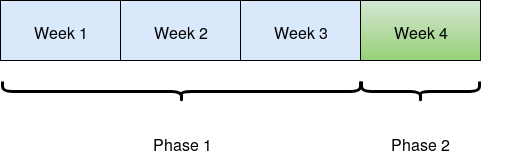
\includegraphics[scale=0.7]{./Figures/study_period.png}
            \caption{Duration and phases of the study period.}
            \label{fig:study-period}
        \end{center}
    \vskip -5mm
\end{figure}

Since the application was openly distributed in Google Play Store, it was possible to make it available to a broader audience. Therefore, additional data were gotten from other people. This data provided extra insights into the use of the application. In this case, the application was advertised in AnkiDroid forums; therefore, it is likely the majority of new users had a previous contact with the original application. Therefore, the information from these new users was isolated from the information from the participants to avoid any incorrect analysis. The users that were not part of the original study were also informed about the nature and objectives of the application.
